\documentclass[type=dr, dr=rernat, accentcolor=tud7b,colorbacktitle, bigchapter, openright, twoside, 12pt ]{tudthesis}
%\documentclass[11pt,twoside,a4paper]{article}
\usepackage[english]{babel} 
\usepackage[utf8]{inputenc}
\usepackage{graphicx}
\usepackage{pstricks}
\usepackage{psfrag}
\usepackage{enumerate}
\usepackage{float}
\usepackage{epsfig}
\usepackage{geometry}
\usepackage{subfigure}
\usepackage{rotating}
\usepackage{minitoc}
% \usepackage{dominitoc}
\usepackage{multirow}
\usepackage{listings}
%\usepackage{appendix}
%\usepackage[breaklinks=true]{hyperref}
%\usepackage{breakcites}

%%%% 1 1/2 facher Zeilenabstand:	
\usepackage{setspace}
\onehalfspacing




\begin{document}
\chapter{Treatment Planning for Patients with multiple lung metastases}
\label{chapter:vmm}
\minitoc

\section{Introduction}

Lung cancer is the leading cause of cancer-related death, with approximately 160 000 deaths in the U.S. in 2014 \cite{Siegel2014}.
More than half of all patients with lung cancer are diagnosed with stage IV non-small cell lung cancer (NSCLC) \cite{Ramalingam2008, Iyengar2014}.
Prognosis for stage IV NSCLC is poor, with only 12 months median survival after first line chemotherapy \cite{Socinski2013}. 

Stereotactic body radiation treatment (SBRT) shows good results for treating NSCLC \cite{Baumann2009, Fakiris2009, Grutters2010, Ricardi2010, Timmerman2010, Greco2011}. 
Furthermore, several studies have shown that SBRT can be used in the setting of limited metastatic 
disease \cite{Rusthoven2009. Villaruz2012, Salama2012, Iyengar2014}. 
Passive scattering particle therapy has also proved as an effective treatment for NSCLC \cite{Grutters2010, Tsujii2012} and it was shown in Chapter~\cite{PatStudy} 
that scanned carbon ions (PT) could also be used as a treatment modality for NSCLC. One of the conclusions of study in Chapter~\ref{PatStudy} 
was that patients with multiple metastases would especially benefit from PT compared to SBRT. However, limitations of this study were small number of patients (4) and single-field uniform optimization (SFUD) used in treatment planning. 
Since patients with multiple metastases can present complex geometry, intensity modulated particle therapy (IMPT) might provide better treatment plan than SFUD.

An investigation of IMPT with state of the art 4D optimization for treating lung cancer patients with multiple metastases was made. Treatment plans were generated with different 4D optimization techniques and compared with
SBRT plans, which were actually used for treating patients.


%A simple geometrical union of target contour in different CT states, geo-ITV, leads to poor 4D dose distribution, when treating moving tumors with particle therapy \cite{Rietzel2010}.

\section{Materials and Methods}

For creation of treatment plans 4D extension of GSI's treatment planning system TRiP98 \cite{Kraemer2000a, Richter2013} was used and modified. A description of modifications and tools used will be given here, 
alongside with patient data and analysis description.

\subsection{Patient data}


In this study, 8 patients with 2 - 5 lung metastases summing to 24 metastases in total were included. The lesion size was 4.2 cm$^3$ (median, 25-75\% 2.4 – 22.2) and peak-to-peak motion was 5.9 mm (2.7 – 8.1). Details are given in Table~\ref{tab:patdata2}.
Target motion and PT treatment planning were based on a 4D-CT, consisting of 10 phases (0 - 9), with phase 0 (end-inhale) chosen as a reference phase.
A registered positron emission tomography (PET) scan was used to delineate clinical target volumes (CTV). 

Patients 1 - 4 had no OARs in CTV vicinity (closer than 10 mm) and patients 5 - 8 had at least one OAR in CTV vicinity (closer than 10 mm).

Patients were treated with SBRT at Chamaplimaud Center for the Unknown, Lisbon (Portugal), with different fraction schemes. Number of fractions and doses delivered are given in Table~\ref{tab:patdata2}. 

\begin{table}[H]
	\centering
	%   \footnotesize
	\caption{Target characteristics, with CTV volumes, peak-to-peak motions, fractionation schemes and number of fields used for treatment planning. Last column 
	shows an OAR in target vicinity (closer than 10 mm). SA stands for smaller airways and esoph. for esophagus.}
	\begin{tabular}{c|c|c|c|c|c|c}
		\hline\hline
		\multirow{2}{*}{Patient} & \multirow{2}{*}{Target} & \multirow{2}{*}{Volume (cm$^3$)} & Peak-to-peak & Fractination & Number & OAR in \\
		 & & & motion [mm] & scheme & of fields & proximity \\
		\hline
		\multirow{2}{*}{1} & a & 10.2 & 3.4  & \multirow{2}{*}{1 x 24 Gy} & \multirow{2}{*}{2} & \multirow{2}{*}{SA} \\
		 & b & 14.4 & 2.8 &  &  &  \\

		 \hline
		 \multirow{2}{*}{2} & a & 2.3 & 12  & 1 x 24 Gy & \multirow{2}{*}{2} \\
		 & b & 0.4 & 11.8  & 5 x 7 Gy &  \\
		 \hline
		 \multirow{5}{*}{3} & a & 3.8 & 5.8  & \multirow{5}{*}{1 x 24 Gy} & \multirow{5}{*}{2} \\
		  & b & 4.3 & 0.8  &  & \\
		  & c & 2.7 & 3.4  &  & \\
		  & d & 3.1 & 2.1  &  & \\
		  & e & 0.5 & 0.5  &  & \\
		  \hline
		  \multirow{2}{*}{4} & a & 139 & 0.6 & \multirow{2}{*}{1 x 24 Gy} & 3 \\
		 & b & 9.2 & 2.0  &  & 2 \\
		 \hline
		 \multirow{2}{*}{5} & a & 4 & 9  & 3 x 9 Gy  & 5 & SA, esoph. \\
		 & b & 0.8 & 7.8  & 1 x 24 Gy & 2 \\
		 \hline
		 \multirow{4}{*}{6} & a & 3.4   & 5    & \multirow{4}{*}{1 x 24 Gy} & 3  \\
				    & b & 2.4 & 4.4  & & \multirow{3}{*}{2} \\
				    & c & 2.0 & 6.3  & & & \multirow{2}{*}{Heart}\\
				    & d & 2.4 & 6.4  & & \\
		\hline	    
		\multirow{2}{*}{7} & a & 20.6 & 7.4 & \multirow{2}{*}{1 x 24 Gy} & \multirow{2}{*}{4} & \multirow{2}{*}{SA}  \\
		 & b & 27.1 & 6.0  &  &   \\
		 \hline
		 \multirow{5}{*}{8} & a & 136 & 12  & 3 x 9 Gy & \multirow{3}{*}{2} & Heart\\
		  & b & 12.4 & 2.5  & 1 x 20 Gy &  &\\
		  & c & 123 & 14  & 3 x 9 Gy &  &Heart \\
		 & d & 80.7 & 17  & 1 x 20 Gy & 3  &\\
		 & e & 86.7 & 6.6  & 1 x 20 Gy & 2 & SA \\
		 
		
		\hline\hline
% 		 
% 		
% 		\hline\hline
	\end{tabular}
	\label{tab:patdata2}
\end{table}

\subsection{Multiple targets}

TRiP98 optimization works on minimizing residual of a nonlinear equation system \cite{Kraemer2000a}. The minimizing function $E(N)$ for particle number $\vec{N}$ goes as:
\begin{equation}
\label{eq-costFunc}
 E(\vec{N}) = \sum_{i\in T} \left( D_{pre}^{i} - D_{act}^{i}(\vec{N})\right) = \sum_{i\in T} \left( D_{pre}^{i} -\sum_{j=1}^n c_{ij}N\right)
\end{equation}

For a CT voxel $i$ in target $T$, $ D_{pre}$ and $D_{act}$ are the prescribed and the actual dose, respectively. The coefficient $c_{ij}$ stands for correlation between dose deposition and field position $j$ at a voxel $i$, 
with $n$ the number of fields. There is no restriction for the number of targets or fields in the minimizing function, so it can be expanded to:

\begin{equation}
\label{eq-multiCost}
 E(\vec{N}) = \sum_{T} \sum_{i\in T} \left( D_{pre}^{i} -\sum_{j=1}^n c_{ij}N\right)
\end{equation}

However, the setup of raster points in TRiP98 allowed only one target. It was therefore expanded in a way that a field was designated to a specific target, as displayed in Fig~\ref{Fig:multiTargets}. 
Raster points for each field are created only around designated target. Contribution from all fields are then calculated in optimization. When a field from one target contributes 
dose to the other target this is taken into account in optimization function, specifically in coefficient $c_{ij}$ in Eq.~\ref{eq-multiCost}. Because the optimization function was not changed, 
all TRiP98 4D functionalities could be used, as explained in next sections.


\begin{figure}[H]
	\begin{center}
		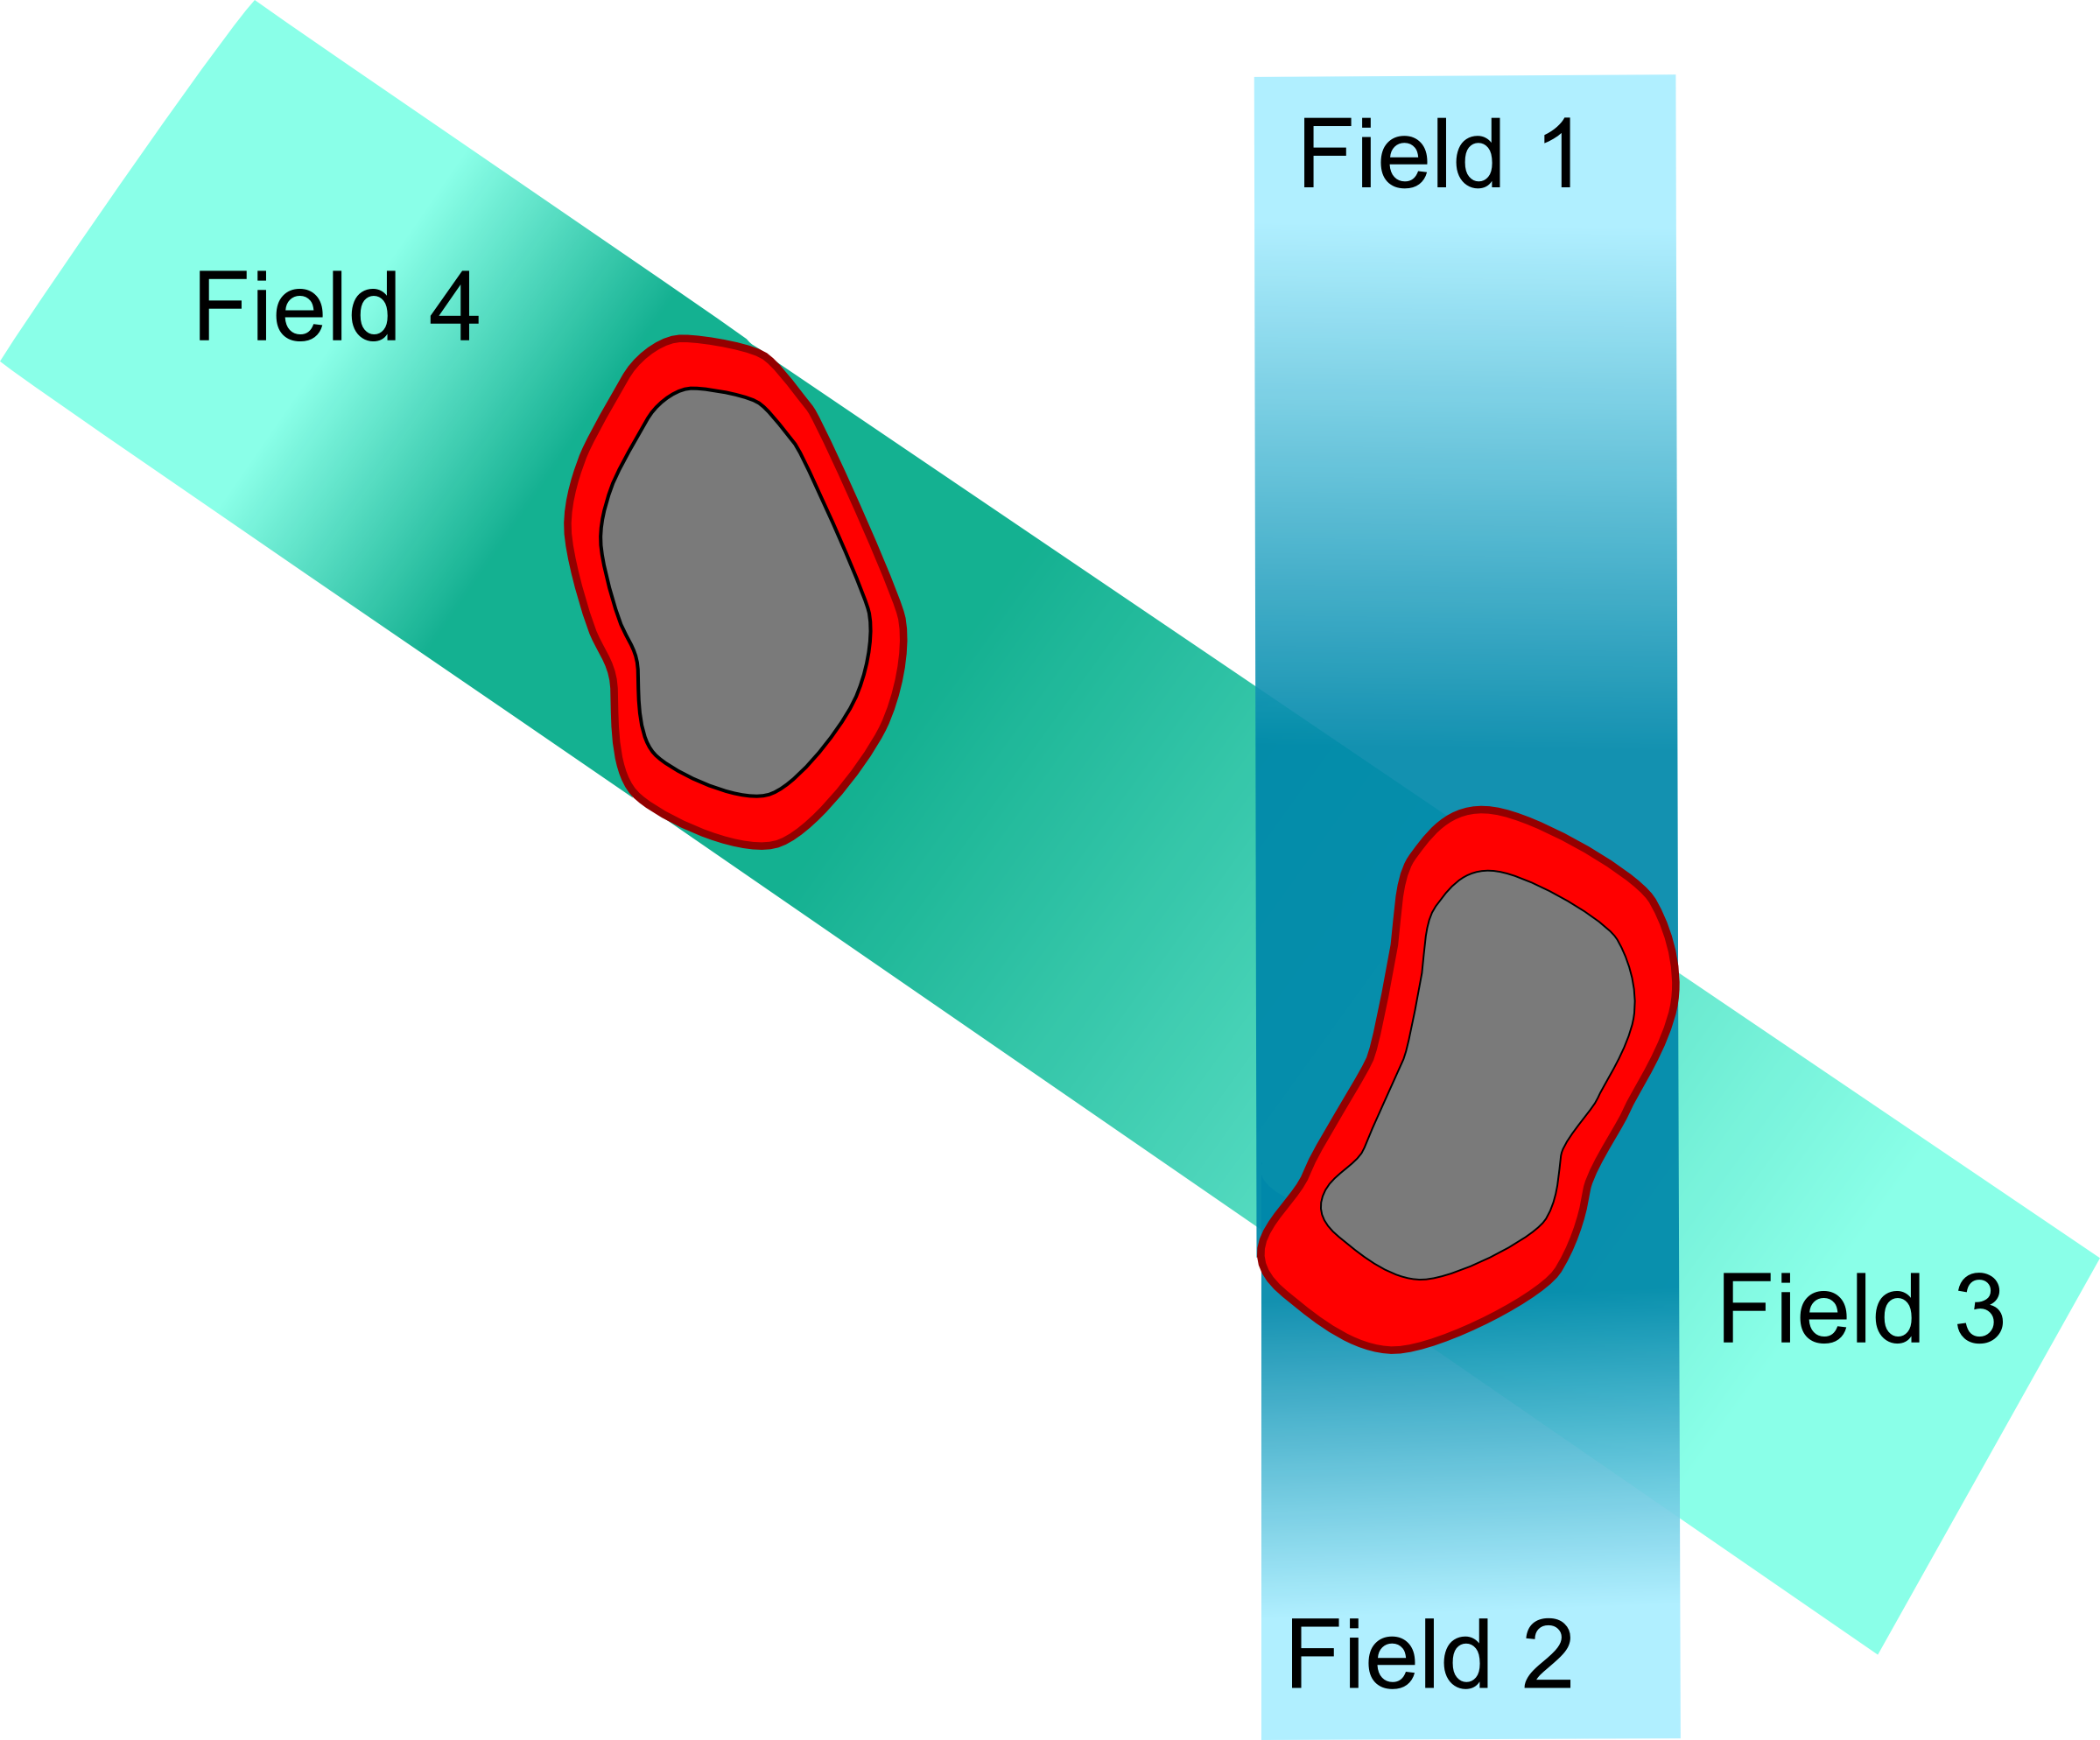
\includegraphics[width=0.7\textwidth]{./Images/multiTarget.png}
		\caption{Multiple targets irradiation. Fields 1 and 2 are designated to target a and fields 3 and 4 to target b. Optimization takes into account all target voxels and contributions from all fields.}
		\label{Fig:multiTargets}
	\end{center}
\end{figure}



\subsection{Optimization techniques}

Investigation of two different optimization techniques to handle range changes in moving tumors was made. For each patient, two sets of plans were created: field-independent ITV (indITV) and 4D optimization (4Dopt). 

\begin{itemize}
\item \textbf{Field-independet ITV:} A water-equivalent path length ITV (WEPL-ITV) is different for each field, creating unnecessary margins when combining WEPL-ITV from different fields (see Fig.~\ref{Fig:weplITV}a). 
Graeff et. al proposed a solution to include range margin into the field description itself, instead of creating a bigger PTV \cite{Graeff2012}. 
Thus, no unnecessary margins are created. Treatment plans were made for all targets with intensity IMPT on a indITV in reference phase.

\item \textbf{4D Optimization:} IMPT with indITV can produce inhomogeneous fields that yield homogeneous dose but only in reference phase. The WEPL can change in different motion phases, leading to inhomogeneous dose.
4Dopt uses WEPL-ITV for raster setup, however the actual optimization is performed on each target voxel in each motion state $k$. The optimization function thus changes to \cite{Graeff2012}:

\begin{equation}
\label{eq-multiCost}
E(\vec{N}) = \sum_{k=1}^{m}\sum_{T_k} \sum_{i\in T_k} \left( D_{pre}^{i} -\sum_{j=1}^n c_{ijk}N\right)
\end{equation}

All targets were treated with IMPT and 4D optimization. A subset of motion states 0, 50 and 70\% was used for targets 7a -7d and 8b (see Table~\ref{tab:patdata2}) due to large optimization problem - beside multiple targets, 
OAR was also included in motion states \cite{Graeff2012}.

\end{itemize}

\begin{figure}[H]
	\begin{center}
		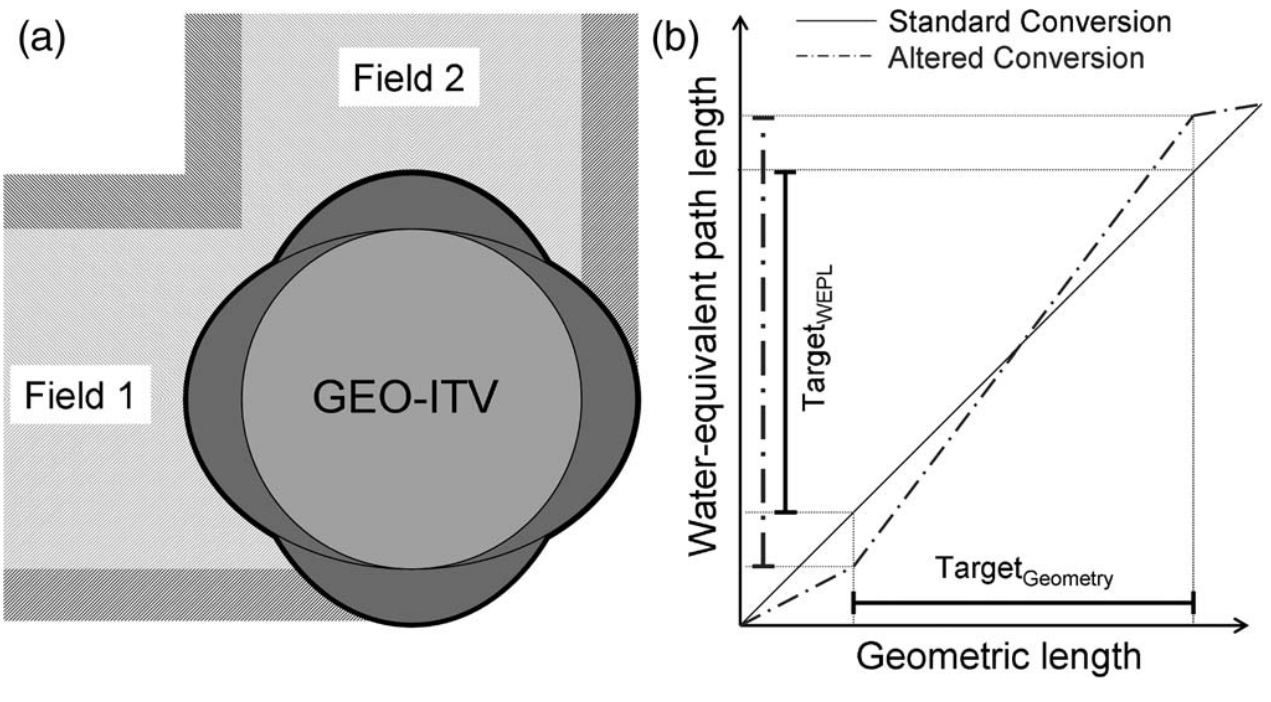
\includegraphics[width=0.7\textwidth]{./Images/weplITV.png}
		\caption{Schematic presentation of the indITV. (a) Dark gray ellipses show margins needed for specific fields to account for range changes in different motion states.
		When common target volume for two perpendicular fields is generated (this black contour) it creates unnecessary lateral extension of both fields, as shown by the dark gray
		entry channels. A solution is shown in (b). Rather than using standard, geometric, margins, both fields use the same geometry, however the conversion of geometry to WEPL
		is altered for each field. The plot in (b) shows the standard (solid line) and an altered conversion (dashed-doted line) for a beam passing a homogeneous CTV. The altered conversion
		increases the WEPL extent and thus implicitly increasing margins for a single field only. Figure taken from \cite{Graeff2012}}
		\label{Fig:weplITV}
	\end{center}
\end{figure}

The same number of fields and the same field angles were used in both techniques.



\subsection{Treatment planning}

An isotropic margin of 3 mm was added to each CTV to account for uncertainties in treatment delivery. An WEPL-ITV was constructed on the CTV with margins for each individual field, which was than used either in optimization (inITV)
or for raster setup (4Dopt). Due to large memory demands, targets in each lung were optimized separately. 
  
The objective for target was 99\% of each target volume should receive at least 100\% of the planned dose (D$_{99}$\% $\geq$ 100\%). Furthermore, the doses to the OARs should be under the limits given by the AAPM task group \cite{Benedict2010}. 
 
After the optimization 4D-dose was calculated for two motion periods (3.6 sec and 5.0 sec) and two starting phases (0$^\circ$ and 90$^\circ$) as explained in Section~\ref{PTTP}. Motion was mitigated with five 
slice-by-slice rescans that were applied to each plan.

Detailed explanation of SBRT treatment planning is given is Section~\ref{SBRTTP}.

For patients 5 - 7 the dose limits to the OARs (stated in Table~\ref{tab:patdata2}) could not be respected by including them in optimization. It was necessary to add margins to the OAR and then 
subtract OAR plus margins from the target.

\section{Results}

Example of different treatment plans for patient 8 is shown in Fig.~\ref{Fig:multiExample}.

\begin{figure}[H]
	\begin{center}
		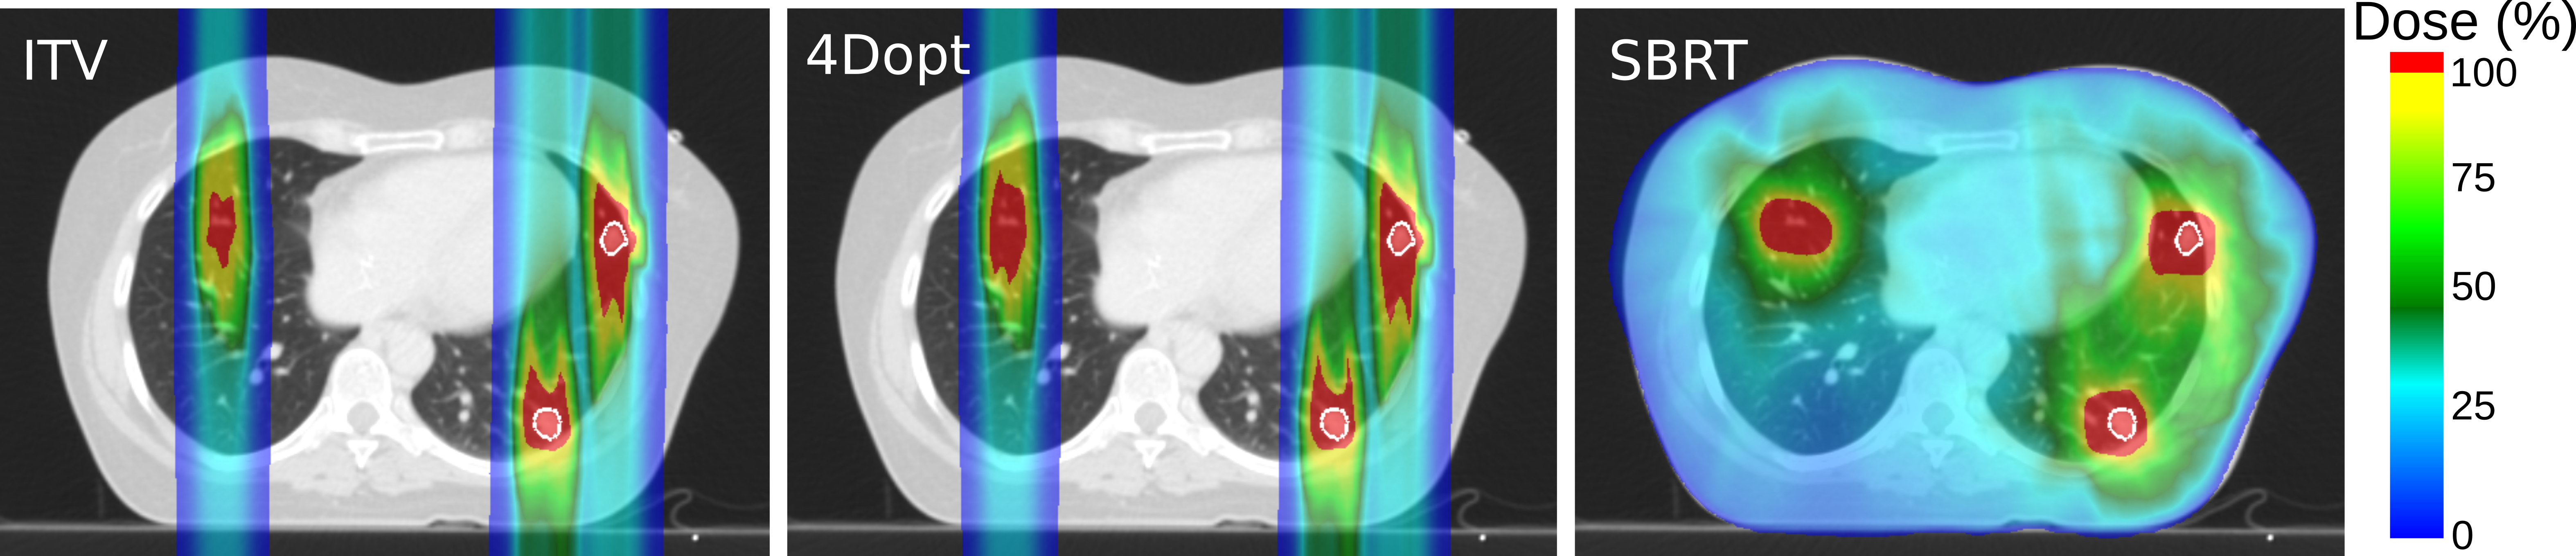
\includegraphics[width=0.9\textwidth]{./Images/multiExample.png}
		\caption{Treatment plans for indITV (left), 4Dopt (middle) and SBRT (right) for SBRT (solid lines) for patients 8. CTV contours are outlined in white.}
		\label{Fig:multiExample}
	\end{center}
\end{figure}

\subsection{Target Coverage}

Results for CTV $D_{99\%}$ for all patients are shown in Table~\ref{tab:resultsComplex}. All SBRT plans were approved by a physician, 
even though the prescription dose for patients 5 - 7 was not met due to an OAR proximity. Excluding patients 5 - 7, there were \textbf{?} cases (out of 20) of too low CTV dose across different
motion types for indITV and 4Dopt, respectively. The lowest CTV $D_{99\%}$ was 98.8\%.
For patients 6 - 8 treatment plans with SFUD were clinically unacceptable, due to violation of OAR constraints. Both indITV and 4Dopt had higher CTV $D_{99\%}$ than SBRT, except for target 7c.
There was no significant difference in target coverage between indITV and 4Dopt. \textbf{SBRT?}

\begin{table}[H]
	\centering
	%   \footnotesize
	\caption{CTV $D_{99\%}$ for indITV, 4Dopt and SBRT for 8 patients. Results for indITV and 4Dopt are shown as median (range) across different motion types.}
	\begin{tabular}{c|c|c|c|c}
		\hline\hline
		\multirow{2}{*}{Patient} & \multirow{2}{*}{Target} & \multicolumn{3}{|c}{CTV $D_{99\%}$} (\%) \\
		 &  & indITV & 4Dopt & SBRT \\
		 \hline
		 
\multirow{2}{*}{1} & a & 101.6(100.0 - 102.1) & 101.0(101.0 - 101.0) & 100.0\\ 
 & b & 101.6(101.0 - 102.1) & 102.1(101.0 - 102.1) & 100.0\\ 
\hline

\multirow{5}{*}{1} & a & 100.9(100.9 - 101.9) & 100.9(100.0 - 100.9) & 105.6\\ 
 & b & 101.3(98.8 - 102.5) & 102.5(100.0 - 102.5) & 105.0\\ 
 & c & 101.4(100.0 - 101.9) & 99.5(99.1 - 100.0) & 106.5\\ 
 & d & 100.6(100.0 - 101.3) & 98.8(98.8 - 101.3) & 112.5\\ 
 & e & 102.5(100.0 - 102.5) & 102.5(101.3 - 102.5) & 101.3\\ 
\hline

\multirow{2}{*}{1} & a & 101.0(100.0 - 101.0) & 100.5(100.0 - 101.0) & 101.0\\ 
 & b & 107.1(103.6 - 107.1) & 100.0(100.0 - 103.6) & 100.0\\ 
\hline

\multirow{5}{*}{1} & a & 101.0(99.0 - 102.1) & 99.0(99.0 - 102.1) & 106.3\\ 
 & b & 102.1(99.0 - 102.1) & 102.1(102.1 - 102.1) & 103.1\\ 
 & c & 101.0(101.0 - 102.1) & 101.6(101.0 - 102.1) & 104.2\\ 
 & d & 102.1(99.0 - 102.1) & 101.6(101.0 - 102.1) & 107.3\\ 
 & e & 102.1(102.1 - 102.1) & 102.1(101.0 - 102.1) & 108.3\\ 
\hline

\multirow{2}{*}{1} & a & 102.1(102.1 - 102.1) & 102.1(102.1 - 102.1) & 101.0\\ 
 & b & 99.0(99.0 - 99.0) & 100.0(100.0 - 101.0) & 102.1\\ 
\hline

\multirow{2}{*}{1} & a & 84.3(82.4 - 85.2) & 69.0(68.5 - 69.4) & 66.7\\ 
 & b & 100.5(99.0 - 102.1) & 100.5(99.0 - 102.1) & 103.1\\ 
\hline

\multirow{4}{*}{1} & a & 100.5(100.0 - 102.1) & 99.5(99.0 - 101.0) & 101.0\\ 
 & b & 100.5(100.0 - 101.0) & 100.0(100.0 - 100.0) & 101.0\\ 
 & c & 91.1(88.5 - 92.7) & 92.7(86.5 - 93.8) & 99.0\\ 
 & d & 97.4(93.8 - 100.0) & 100.0(99.0 - 101.0) & 94.8\\ 
\hline

\multirow{2}{*}{1} & a & 87.5(86.5 - 89.6) & 94.3(92.7 - 94.8) & 69.8\\ 
 & b & 79.7(79.2 - 81.3) & 78.6(77.1 - 79.2) & 69.8\\ 
\hline

		
		\hline




		\hline
		
% 		\hline\hline
	\end{tabular}
	\label{tab:resultsComplex}
\end{table}

% \newpage
% 
% \begin{table}[H]
% 	\centering
% 	%   \footnotesize
% 	\caption{Target characteristics, with CTV volumes, peak-to-peak motions, fractination schemes and number of fields used for treatment planning.}
% 	\begin{tabular}{c|c|c|c|c|c}
% 		\hline\hline
% 		\multirow{2}{*}{Patient} & \multirow{2}{*}{Target} & \multicolumn{4}{|c}{D$_{99\%}$} \\
% 		 & & SFUD & indITV & 4Dopt & SBRT \\
% 		\hline
% \multirow{2}{*}{1} & a & 101.0(100.0 - 101.0) & 101.0(100.0 - 102.1) & 101.0(101.0 - 101.0) & 100.0\\ 
%  & b & 102.1(102.1 - 102.1) & 101.6(101.0 - 102.1) & 101.0(101.0 - 102.1) & 100.0\\ 
% \hline
% 
% \multirow{5}{*}{1} & a & 104.2(101.9 - 105.6) & 100.9(100.0 - 101.9) & 100.0(99.1 - 100.0) & 100.9\\ 
%  & b & 101.9(101.3 - 103.8) & 100.6(98.8 - 101.3) & 101.3(100.0 - 101.3) & 92.5\\ 
%  & c & 114.4(113.9 - 114.8) & 100.9(100.0 - 101.9) & 99.1(98.1 - 100.0) & 106.5\\ 
%  & d & 98.1(97.5 - 98.8) & 100.0(98.8 - 101.3) & 98.1(97.5 - 100.0) & 112.5\\ 
%  & e & 101.3(101.3 - 101.3) & 102.5(100.0 - 102.5) & 101.3(101.3 - 102.5) & 81.3\\ 
% \hline
% 
% \multirow{2}{*}{1} & a & 99.5(95.8 - 101.0) & 100.0(99.0 - 101.0) & 100.0(100.0 - 100.0) & 101.0\\ 
%  & b & 96.4(92.9 - 103.6) & 103.6(100.0 - 103.6) & 100.0(100.0 - 103.6) & 100.0\\ 
% \hline
% 
% \multirow{5}{*}{1} & a & 99.5(97.9 - 100.0) & 100.5(99.0 - 101.0) & 97.9(97.9 - 100.0) & 106.3\\ 
%  & b & 100.0(100.0 - 100.0) & 102.1(94.8 - 102.1) & 101.0(101.0 - 101.0) & 103.1\\ 
%  & c & 100.5(100.0 - 101.0) & 100.5(99.0 - 102.1) & 101.0(100.0 - 101.0) & 104.2\\ 
%  & d & 94.3(93.8 - 94.8) & 102.1(95.8 - 102.1) & 101.0(101.0 - 101.0) & 107.3\\ 
%  & e & 94.8(94.8 - 94.8) & 100.5(100.0 - 101.0) & 100.0(99.0 - 100.0) & 108.3\\ 
% \hline
% 
% \multirow{2}{*}{1} & a & 102.1(102.1 - 102.1) & 100.0(100.0 - 100.0) & 100.0(100.0 - 100.0) & 101.0\\ 
%  & b & 97.4(96.9 - 97.9) & 96.9(96.9 - 97.9) & 94.8(94.8 - 94.8) & 102.1\\ 
% \hline
% 
% \multirow{2}{*}{1} & a & 84.3(83.3 - 85.2) & 72.7(72.2 - 73.1) & 56.0(55.6 - 56.5) & 0.0\\ 
%  & b & 82.8(80.2 - 85.4) & 100.0(96.9 - 101.0) & 99.0(99.0 - 99.0) & 101.0\\ 
% \hline
% 
% \multirow{4}{*}{1} & a & 101.0(99.0 - 102.1) & 100.0(99.0 - 101.0) & 97.4(96.9 - 97.9) & 101.0\\ 
%  & b & 106.8(105.2 - 107.3) & 97.9(96.9 - 99.0) & 96.4(95.8 - 96.9) & 101.0\\ 
%  & c & 97.9(97.9 - 99.0) & 69.3(68.8 - 70.8) & 66.7(63.5 - 68.8) & 85.4\\ 
%  & d & 100.0(99.0 - 101.0) & 71.9(70.8 - 72.9) & 72.9(70.8 - 75.0) & 83.3\\ 
% \hline
% 
% \multirow{2}{*}{1} & a & 85.9(85.4 - 86.5) & 69.3(68.8 - 70.8) & 72.9(72.9 - 74.0) & 58.3\\ 
%  & b & 68.2(66.7 - 69.8) & 62.0(60.4 - 62.5) & 57.3(57.3 - 58.3) & 53.1\\ 
% \hline
% 
% 		
% 		\hline
% 	\end{tabular}
% 	\label{tab:resultsComplex2}
% \end{table}

\subsection{Dose in OARs}

$D_{Max}$ and $D_{Mean}$ for 8 OARs are shown in Table~\ref{tab:OARComplex}. There was a significant difference between PT and SBRT in $D_{Max}$ and $D_{Mean}$ for heart, spinal cord, esophagus and aorta and in $D_{Mean}$ for ipsilateral lung.
No significant difference was observed in dose to OAR between different motion types or between indITV and 4Dopt. $D_{Max}$ to all OARs was \textbf{?} and and for indITV, 4Dopt and SBRT, respectively.

DVHs for patients 5 - 8 are shown in Fig.~\textbf{Do it!}. The margins used for OAR subtraction for PT and SBRT, respectively, were:
0 and 5 mm for smaller airways, 0 and 1 mm for esophagus in patient 5; 
0 and 2 mm for heart in patient 6; 
2 and 11 mm for smaller airways in left lung, 0 and 9 mm for smaller airways in right lung.

$D_{Max}$ limit for smaller airways was exceeded for patients 5 and 7 and heart $D_{Max}$ limit for patient 7 in all cases. For patient 5 the indITV plan was clinically unacceptable, 
due to too large dose to 0.5 cm$^3$ volume of smaller airways (19.6 Gy compared to 15.1 Gy and 15.3 Gy from 4Dopt and SBRT, respectively).


\begin{table}[H]
	\centering
	%   \footnotesize
	\caption{Target characteristics, with CTV volumes, peak-to-peak motions, fractination schemes and number of fields used for treatment planning.}
	\begin{tabular}{c|c|c|c|c}
		\hline\hline
		OAR & SFUD & indITV & 4Dopt & SBRT \\
		\hline
heart & 0.4(0.0 - 1.1) & 0.3(0.0 - 0.8) & 0.4(0.0 - 1.0) & 4.4(2.5 - 10.1)  \\ 
spinalcord & 0.0(0.0 - 0.7) & 0.0(0.0 - 0.5) & 0.0(0.0 - 0.6) & 1.8(0.8 - 2.5)  \\ 
smallerairways & 0.3(0.0 - 10.4) & 1.1(0.0 - 8.2) & 1.2(0.0 - 10.3) & 3.5(0.0 - 7.5) \\ 
esophagus & 0.1(0.0 - 1.5) & 0.1(0.0 - 1.4) & 0.1(0.0 - 1.8) & 3.3(1.4 - 5.1)  \\ 
trachea & 0.0(0.0 - 0.1) & 0.0(0.0 - 0.0) & 0.0(0.0 - 0.1) & 0.1(0.0 - 3.0)  \\ 
aorta & 0.5(0.0 - 1.1) & 0.4(0.0 - 1.0) & 0.5(0.0 - 0.8) & 2.9(1.3 - 6.2)  \\ 
lungl & 3.5(0.1 - 11.0) & 3.0(0.0 - 9.1) & 3.0(0.1 - 8.6) & 5.9(0.9 - 10.5)  \\ 
lungr & 2.0(0.0 - 3.3) & 1.8(0.0 - 6.0) & 1.9(0.0 - 5.6) & 3.0(0.8 - 8.6)  \\ 

\hline\hline

heart & 14.1(0.0 - 39.3) & 13.9(0.0 - 28.5) & 14.6(0.0 - 29.3) & 18.1(7.5 - 30.5)\\ 
spinalcord & 0.4(0.0 - 8.0) & 0.4(0.0 - 8.3) & 0.3(0.0 - 8.5) & 9.0(3.0 - 12.5)\\ 
smallerairways & 14.1(0.0 - 26.0) & 13.5(0.0 - 24.0) & 13.8(0.0 - 27.5) & 15.6(0.0 - 22.8)\\ 
esophagus & 0.6(0.0 - 23.8) & 0.6(0.0 - 23.5) & 1.0(0.0 - 26.0) & 11.5(5.5 - 25.5)\\ 
trachea & 0.0(0.0 - 3.8) & 0.0(0.0 - 1.3) & 0.0(0.0 - 5.0) & 0.4(0.0 - 7.5)\\ 
aorta & 6.9(2.0 - 35.8) & 4.6(0.0 - 28.5) & 6.5(1.5 - 26.5) & 18.1(6.3 - 31.0)\\ 
lungl & 26.8(8.0 - 52.3) & 27.1(0.0 - 31.5) & 26.6(8.0 - 29.8) & 26.5(10.0 - 32.3)\\ 
lungr & 26.0(0.3 - 30.5) & 25.8(0.5 - 34.8) & 26.1(0.3 - 29.0) & 26.1(3.8 - 30.0)\\ 
\hline\hline

	\end{tabular}
	\label{tab:OARComplex}
\end{table}


\section{Summary and Discussion}

Clinically valid SBRT plans have been compared to PT treatment plans for NSCLC patients with multiple metastases. 
To the best of our knowledge, this is the first study of treating multiple NSCLC metastases with PT. Novel approach was used to handle multiple targets, together
with the state of the are 4D PT treatment planning. Furthermore, 4D PT doses were calculated for different motion types. 

PT on average delivered less dose to OAR, while still having comparable target coverage.
The most apparent difference is in lung $V{_20\%}$, which was 3333\% lower in PT, due to the narrow entry channel PT use.
For patients 5 - 8, PT maintained or even improved target coverage, while reducing $D_{Mean}$ to OARs. Additionally,  margins used for OAR subtraction were smaller in PT.

There was no significant difference between indITV and 4Dopt in target coverage or in dose to OAR. However, in patients 5 - 8 the 4Dopt was able to have higher target coverage, while respecting the OAR dose limits.

Even though PT deposit less dose to OAR with the same or even better target coverage, there is still room for improvement in PT 4D treatment planning. 
An implementation of multi-criteria objective planning should bring even better dose distribution and bring possibility to choose between trade-offs \cite{Breedveld2007, Chen2010}.
Additionally, multiple target optimization in PT would benefit from a shell around PT where dose would be minimized. Therefore excessive dose
in healthy tissue would be further reduced. An introduction of a shell, however, would further enlarge the optimization problem, which is big already for complex geometry (patient 5 - 8). 
A solution for minimizing voxel number in optimization is currently being implemented by Prall et al \textbf{Citat, mogoce mal vec napisat.} 

In Chapter~\ref{PatStudy} additional range margins to account for range uncertainties could be used in treatment planning, due to SFUD. 
Because we did not use field specific PTVs it was not possible to include range uncertainties in our study.
Instead of creating field specific PTVs to include range uncertainties, a solution was proposed to include uncertainties in optimization process itself \cite{Pflugfelder2008, Unkelbach2009, Fredriksson2011, Chen2012}.
Chen et al. have shown it is possible to implement robust optimization in multi-criteria optimization as well \cite{Chen2012}. Furthermore, in a recent treatment planning study by Liu et al. \cite{Liu2016}
a 4D robust optimization was demonstrated, with better results over 3D robust optimization for NSCLC patients. However, only breathing starting phase was used as an uncertainty,
whereas different motion types should be considered. Patient 6 $D_{Max}$ heart dose ranged over 2 Gy across different motion types in 4Dopt, showing the necessity of making treatment plans robust against motion uncertainty, 
especially in the hypo-fractionated regiment. The disadvantage of 3D and 4D robust optimization is the enlargement of the optimization problem.

Apart from 4D robust optimization, the effect of motion could be minimized by using other motion mitigation techniques, such as gating. Furthermore, gating could improve the target coverage, where the planned dose was
not met. Gating, together with rescanning, has already been successfully implemented clinically for active beam scanning \cite{Rossi2016, Mori2016} and it might be essential to use it in hypo-fractionated 
treatment of moving tumors.

A recent review showed good local control rates between 66 - 92\% for patients treated with SBRT in reoccurred tumors in previous irradiation field \cite{Amini2014}. 
However, there were grade 4 and 5 complications present, i.e. study by Trovo et al showed grade 5 pneumonia in
6\% of patient treated \cite{Trovo2014}. As shown in our study, PT delivers less dose to the OAR and could hence reduce the number of complications.

\section{Conclusions}

PT delivers less dose to OAR compared to SBRT in NSCLC patients with multiple disease sites, while maintaining the same target coverage. 
Caution has to be taken in patients with OAR in CTV vicinity (less than 10 mm), where doses to OAR differ across different motion types.
No significant difference was found between two 4D optimization techniques. However, 4D optimization showed better results for patients with OAR in CTV vicinity.




\bibliographystyle{apalike}
\bibliography{../ref.bib}{}
% \bibliographystyle{plain}

\end{document}